\chapter{Caminatas cuánticas sobre gráficas}

\section{Sobre el plano infinito}
Las caminatas sobre el plano infinito construido con rejilla cuadrada. Con tres monedas distintas la dispersión de

\subsubsection*{Grover}
\begin{equation}
H=\frac{1}{2}
\begin{pmatrix}
-1 & 1 & 1 & 1\\
1 & -1 & 1 & 1\\
1 & 1 & -1 & 1\\
1 & 1 & 1 & -1
\end{pmatrix}
\qquad ; \qquad    \ket{\Psi(0)}=\frac{1}{2}(\ket{00}-\ket{01}-\ket{10}+\ket{11})\otimes\ket{x=0,y=0}
\end{equation}{}

\begin{figure}[ht]
\caption{}
\centering
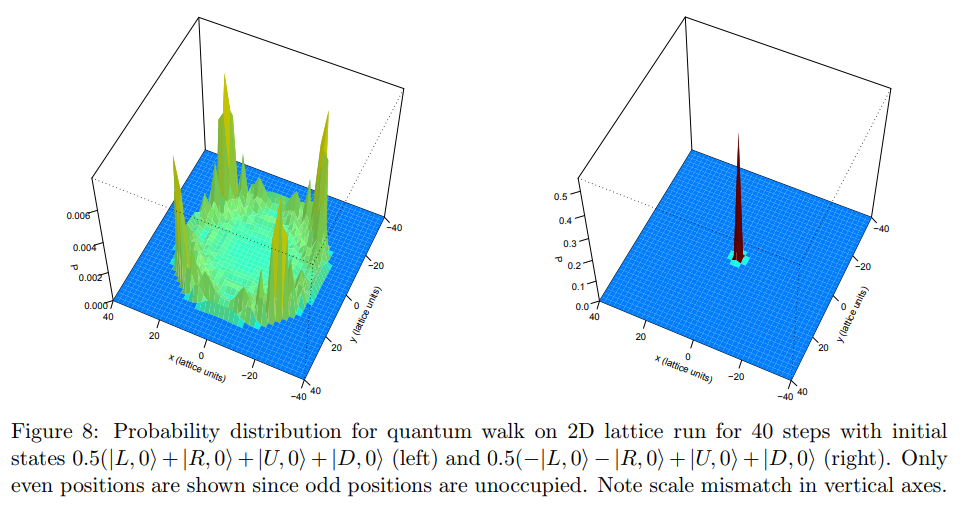
\includegraphics[width=0.5\textwidth]{QWGroverCoinKendonPercolation2019.png}
\end{figure}

\section{Gráficas finitas}
En el análisis de la dinámica definimos el \textit{periodo} y \textit{cuasi-periodo} de la distribución y damos las razones por las cuales no es posible converger a una distribución límite, a diferencia del caso clásico\cite{aharonov2001quantum}. Sin embargo, es usual el trabajo con una distribución promedio sobre las distribuciones originales que elimina la 'memoria' de los estados iniciales en el sistema permitiendo alcanzar una distribución estacionaria límite sobre esta nueva distribución. Introducimos los conceptos de \textit{mixing time} y \textit{hitting time} que descatan diferencias adicionales entre las caminatas, y más importante aún, descatan las ventajas (la mayoría de veces) de las caminatas cuánticas sobre las clásicas en la implementación de algoritmos.\\

El estudio sobre gráficas regulares finitas de clase 1 se puede generalizar a gráficas de clase 2 \cite{portugal2013quantum}.

\subsection{Definiciones básicas}

La evolución es la operación repetida de la moneda $\hat{C}$ y la traslación $\hat{S}$.
$\hat{U}=\hat{S}(\hat{C}\otimes I)$.
\begin{equation*}{}
\hat{S}\ket{j}\otimes\ket{v}=
    \left\{
    \begin{array}{cl}
    \ket{j}\otimes\ket{w}    & \text{if}\,\;\;\;\;e^j_v=(v,w) \\
    0  & \text{otherwise}
    \end{array}{}
    \right.
\end{equation*}{}
\subsection{Dinámica del sistema}

\noindent\textbf{Definición} Una caminata cuántica on base en la evolucíón por pasos $\ket{\psi(t)}=\hat{U}^t\ket{psi(0)}$ es \textit{periódica} si existe un \textit{periodo fundamental} $t_0\in\mathcal{Z}^+$ y un ángulo $\alpha$ tal que $\hat{U}^{t_0}=e^{i\alpha}\mathcal{I}$. Esto significa que $|\braket{\Psi(nt_0)|\Psi(0)}|^2=1$ para $n$ entero.\\

\noindent\textbf{Definición} Una caminata cuántica con base en la evolución $\ket{\psi(t)}=\hat{U}^t\ket{\psi(0)}$ tiene dinámica \textit{cuasi periódica} si para cualquier $\epsilon\in\mathbb{R}^+$, hay un tiempo $t$ tal que $||\hat{U}-\mathcal{I}||\leq\epsilon$.
Esto implica que para cualquier $\epsilon$ fijo, hay $t$ tal que $|\braket{\psi(t)|\psi(0)}|\geq1-\epsilon$.\\
En \cite{aharonov2001quantum} se lleva a cabo la estrategia para calcular la distribución límite para el N-círculo, equivalente para otras gráficas.\\
Dada la evolución unitaria de un sistema cuántico, siempre es posible su evolución contraria, porque a cada paso existe $\hat{U}^{-1}$ que revierte $\hat{U}$. Entonces la distribución después de muchos pasos depende de la estado inicial. Consideramos la distribución límite como la distribución uniforme sobre las distribuciones de probabilidad para cada estado inicial posible.\\

¿Existe el límite $\lim_{t\xrightarrow{}\infty}\ket{\psi(t)}$? Es posible una respuesta demostrando que la dinámica de las caminatas cuánticas sobre gráficas finitas es cuasi-periódica. Demos unas definiciones y el teorema correspondiente. "hay infinito número de tiempos een que el estado cuántico está cerca al estado inicial, presentando una estructura repetitiva en las escalas de tiempo."\\


\subsubsection{Algunas gráficas}

\subsubsection*{Ciclo}
Un N-ciclo tiene N vértices y condiciones de frontera periódicas, es decir, el vértices de los extremos coinciden y son el mismo. Un caminante sobre un vértices de un N-ciclo puede tomar dos direcciones: a favor o en contra de las manecillas del reloj. En el modelo de moneda, sus estados son $\{\ket{j,v}|j=0,1;v=0,\dots,N-1\}$.
\begin{equation}
    \hat{S}\ket{j,v}\xrightarrow{}\ket{j}\ket{j,v+(-1)^j}
\end{equation}{}
$v$ se incrementa si $j=0$. Usamos $\hat{H}$ para la evolución $\hat{U}=\hat{S}(\hat{H}\otimes I)$. Por la simetría espacial, la transformada de Fourier facilita la expresión que resulta de la operación de $\hat{U}$, en particular, los autoestados de $\hat{S}$
son los estados de la base ortnormal de Fourier $\{\widetilde{\ket{k}}|k\in [-\pi,\pi] \}$. Esto reduce el problema a diagonalizar $\hat{H}$, para obtener finalmente el espectro de la evolución:
\begin{equation}
    \hat{U}^t=\int_{-\pi}^\pi\frac{dk}{2\pi}\left(e^{-i\theta_kt}\ket{\alpha_k,\widetilde{k}}\bra{\alpha_k,\widetilde{k}}+e^{i(\pi+\theta_k)t}\ket{\beta_k,\widetilde{k}}\bra{\beta_k,\widetilde{k}}\right)
\end{equation}{}
Hallamos $\ket{\psi(t)}=\hat{U}^t\ket{\psi(0)}$ con la condición inicial $\ket{\psi(0)}=\ket{0}\ket{0}$, que es moneda a contrarreloj y posición del vértice $0$:

\begin{equation}
\ket{\psi(t)}=\dfrac{1}{N}    \sum_{j,k}A_k(t)e^{2\pi ikj/N}\ket{j}+\dfrac{1}{N}    \sum_{j,k}B_k(t)e^{2\pi ikj/N}\ket{j}
\end{equation}
donde $j$ y $k$ recorren todas las posiciones,

\begin{align}
    A_k=\cos\theta_k t-\dfrac{i\cos\kappa\sin\theta_kt}{\sqrt{1+\cos^2\kappa }}
    B_k=\dfrac{-ie^{i\kappa}\sin\theta_kt}{\sqrt{1+\cos^2\kappa}}
\end{align}
con $\kappa=2\pi k/N$. La probabilidad de estar en $j$ es

\begin{equation}
    P_j=\dfrac{1}{N}|\sum_{k}A_k(t)e^{2\pi ikj/N}|^2+\dfrac{1}{N}|\sum_{k}B_k(t)e^{2\pi ikj/N}|^2
\end{equation}
Estas ecuaciones son válidas para cualquier N, pero sólo para tiempos $t$ pares. Cuando $t$ es impar, intercambiamos $\cos\theta_k\xrightarrow{}-i\sin\theta_k$ en $A_k$ y $B_k$. 
En el N-ciclo los frentes de onda no se alejan siempre como en la línea infinita, por el contrario se acercan, y en $t\approx N/2$ se encuentran. Cuando $N$ es par las dos ondas interfieren sobre los puntos pares, en particular, en $N/2$. Por el contrario, para $N$ impar las ondas se entrecruzan en las posiciones, es decir, se dispersan sobre toda la gráfica pero sin tocarse, ya que para cualquier tiempo la posición de un frente son los impares mientras que para la otras son los pares. En tiempos grandes, para $N$ par y $t+j$ impar la probabilidad es nula, eso no es cierto en general para $N$ impar. Esta diferencia se evidencia mayormente en la distribución límite: que es uniforme e independiente para casos impares, y no uniforme y dependiente de las condiciones iniciales para ciclos pares.
Las interferencias introducidas a través de $\hat{H}$ no pueden ser reproducidas escogiendo adecuadamente las condiciones iniciales como en el caso de la línea infinita (ver sección (\ref{sec:Moneda})).\\

El periodo $T$ puede ser calculado a partir de $\hat{U}^T=I$, de lo cual se desprende que los autovalores de $\hat{U} $ a la potencia $T$ son $1$: $e^{-i\theta_k T}=e^{i(\pi+\theta_k)T}=1$ para todo $k$, cuyas soluciones más pequeñas son: $N=2,\, T=2$, $N=4,\,8$, $N=8,\,T=24$, $\dots$.

\begin{figure}[ht]
\centering
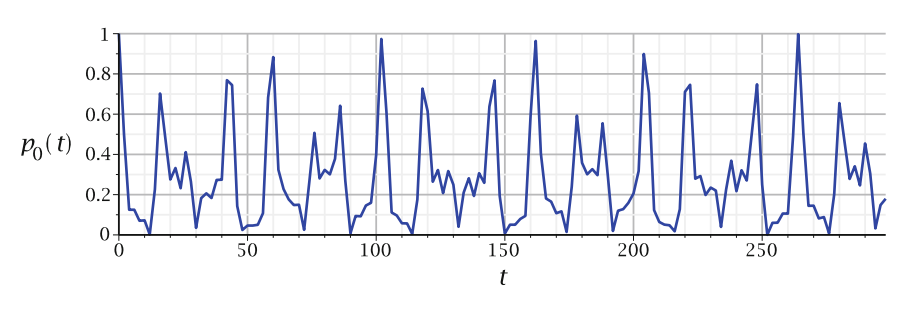
\includegraphics[width=0.8\textwidth]{Kap4/Quasiperiodyc10CyclePortugal.png}
\caption{Distribución del vértice $v=0$ en un 10-ciclo. En $t=264$ la probabilidad es muy cercana a $1$. Asimismo en otros tiempos la distribución es muy próxima a $1$.
\cite{portugal2013quantum}}
\end{figure}

\begin{equation}
    \Vec{c}^t=\frac{1}{t}\sum_{s=1}^t\Vec{p}^s
\end{equation}{}
\begin{equation}
c_i^t=\dfrac{1}{t}\sum_{s=1}^t\sum_{\alpha=\uparrow.\downarrow}\sum_{k,l=1}^{2N}a_ka_l*(\lambda_k\lambda_l*)^s\braket{\alpha,i|v_k}\braket{v_l|\alpha,i}
\end{equation}{}
\begin{equation}
    c_i^t\xrightarrow{t\xrightarrow{}\infty}\sum_{\alpha=\uparrow,\downarrow}\sum_{k,l=1}^{2N}a_ka_l^*\braket{\alpha,i|v_k}\braket{v_l|\alpha,i}=:\Vec{\pi_i}
\end{equation}{}


\subsubsection*{Gráfica 2D finita}
Una red 2D con condiciones de frontera periódicas corresponde a un \textit{toro}. Si la red tiene $N$ vértices, y sus lados $\sqrt{N}$, los estados en el modelo de moneda son $\{\ket{d,s}\otimes\ket{x,y}d,s=0,1,x,y=0,\dots \sqrt{N}-1\}$ en donde los estados de las monedas $\ket{d,s}$ están en $\mathcal{H}^2\otimes \mathcal{H}^2$, y son tales que $d$ designa el eje de movimiento: $d=0$ sobre el eje $x$, y $d=1$ sobre $y$, y si $s=0$ la dirección es hacia los negativos, y si $s=1$ hacia los positivos. Los estados de posición están en  $\mathcal{H}^{\sqrt{N}} \otimes   \mathcal{H}^{\sqrt{N}}$. La evolución $\hat{U}=\hat{S}\hat{C}$:

\begin{equation}
    \hat{S}\ket{d,s}\ket{x,y}\xrightarrow{}\ket{d,s}\ket{x+(-1)^{\delta_{0,s}},y+(-1)^{\delta_{1,s}}}
\end{equation}{}

\begin{equation}
    \ket{\psi(t)}=\dfrac{1}{\sqrt{N}}\ket{D}\ket{D}+\dfrac{1}{\sqrt{2N}}\sum_{\begin{array}{c} k,l=0\\ (k,l)\neq(0,0) \end{array}}^{\sqrt{N}-1} (e^{i\theta_klt}\ket{\nu_{kl}^{\theta}}+e^{-i\theta_klt}\ket{\nu_{kl}^{-\theta}})
\end{equation}
donde $\theta_{kl}=\frac{1}{2}(\cos{\dfrac{2\pi k}{\sqrt{N}}}+\cos{\dfrac{2\pi l}{\sqrt{N}}})$, y 
\begin{equation}
    \ket{\nu_{kl}^{\pm\theta}}=\dfrac{i}{2\sqrt{2}\sin{\theta_{kl}}}
      \left(
    \begin{array}{c}
        e^{i\theta_{kl}}-\omega^k   \\
        e^{-i\theta_{kl}}-\omega^{-k}\\
        e^{-i\theta_{kl}}-\omega^{l}\\
        e^{-i\theta_{kl}}-\omega^{-l}
    \end{array}
    \right)
\end{equation}
\subsubsection*{Hipercubo}
[17 en Kempe] Calculate the expected hitting time where an exponential speed up is reached. 
We have that the hypercube doesn't mixed at all in continuous quantum walk.
\cite{marquezino2008mixing}
\subsubsection*{Gráfica de árboles ligados}

\begin{figure}[ht]
\centering
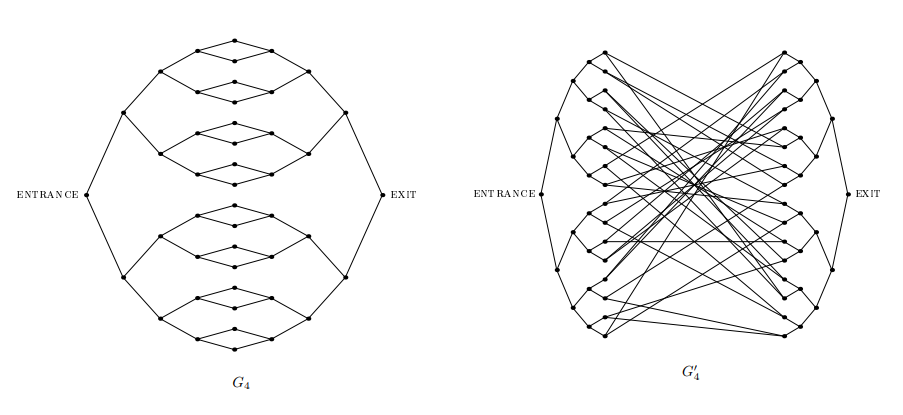
\includegraphics[width=1\textwidth]{Kap4/GluedTreesChilds.png}
\caption{La distancia de la mitad no es importante, sirve para esclarecer la imagen.  $G_n$ es más sencilla que $G_n'$.  \cite{childs2003exponential}}
\end{figure}

[Childs] [Fahri] analizaron la gráfica de árboles ligados con profundidad $n$, $G_n$, y compararon el \textit{hitting time} promedio con el caso clásico. Con la caminata en tiempo continuo obtuvieron una mejora en exponencial. 
\begin{figure}[ht]
\centering
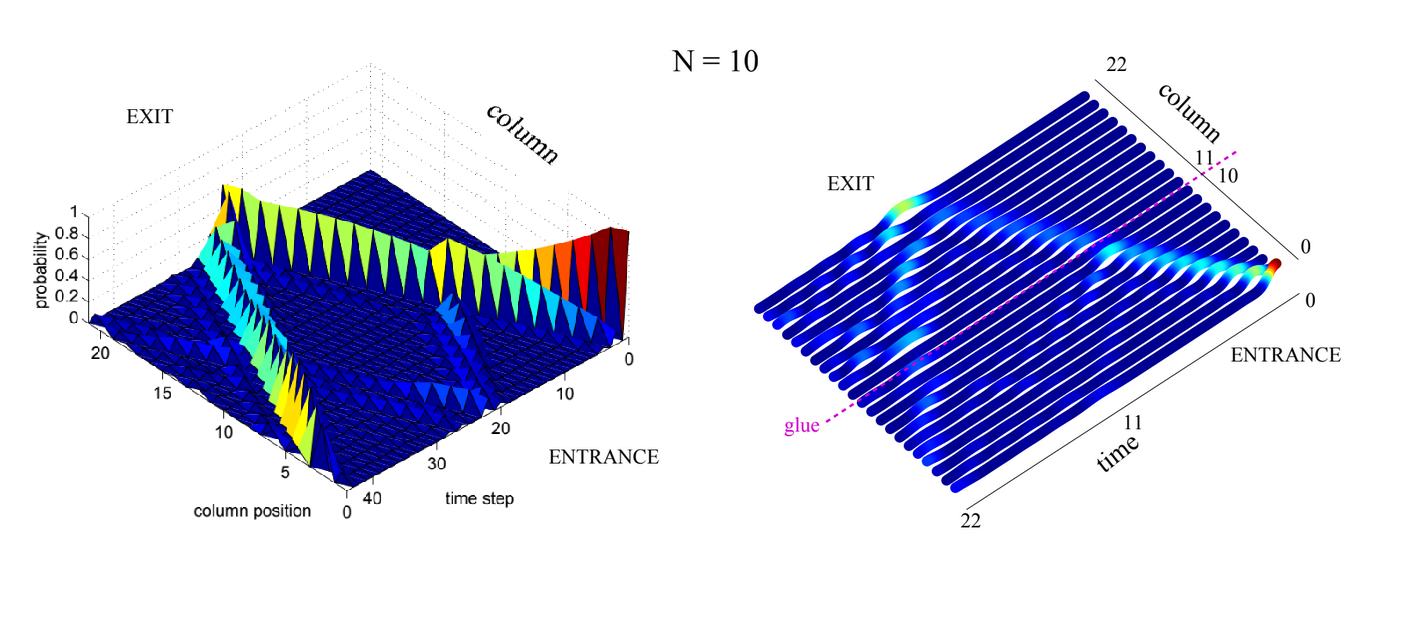
\includegraphics[width=1\textwidth]{Kap4/GluedTreesCarneiro.png}
\caption{Caminata de tiempo continuo en el que $G_4$, para $N=10$. \cite{carneiro2005entanglement}}
\end{figure}

\begin{equation*}
    \ket{\text{col}\,j}=\dfrac{1}{\sqrt{N_j}}\sum_{v\,\in \, \text{column}\,j} \ket{v},
\end{equation*}{}

where

\begin{equation*}
    N_j=
    \left\{
    \begin{array}{ll}
    2^j & 0\leq j\leq n\\
    2^{2n+1-j} & n+1\leq j \leq 2n+1
    \end{array}
    \right.
\end{equation*}{}
\begin{equation*}
    \bra{\text{col}\,j}H\ket{\text{col}\,(j+1)}=
    \left\{
    \begin{array}{ll}
    \sqrt{2}\gamma     & 0\leq j\leq n-1\,,\,\,\,n+1\leq j\leq 2n  \\
    2\gamma     & j=n 
    \end{array}{}
    \right.
\end{equation*}{}

\begin{equation*}
    \braket{j|p}=\dfrac{1}{\sqrt{2\pi}}e^{ipj},\,\,\,\,\,\,-\pi\leq p\leq\pi
\end{equation*}{}
having energies $E_p=2\cos p$
\begin{align*}
    G(j,k,t)&=\bra{k}e^{-i\hat{H}t}\ket{j}\\
    &=\dfrac{1}{2\pi}\int_{-\pi}^{\pi}dp e^{ip(k-j)-2it\cos p}\\
    &=(-i)^{k-j}J_{k-j}(2t), \,\,\,\,\,\, -\infty < j,k < \infty
\end{align*}{}

\begin{align}
    J_\nu(\nu/\cosh{\zeta})
\end{align}{}

La probabilidad de estar en la raíz derecha habiendo partido de la raíz izquierda es:
\begin{equation}
    \Vec{\pi}\geq \frac{1}{2n+1},
\end{equation}
por su parte en el caso clásico:
\begin{align}
    \pi_b&=\lim_{t\xrightarrow{}\infty} p_b(t),
    \pi_b&=(2^{n+1}+2^n-2)^{-1}\\
\end{align}
\cite{childs2002example}


%\begin{figure}[ht]
%\caption{addfad}
%\centering
%\includegraphics[width=0.5\textwidth]{.png}
%\end{figure}
